The analysis uses a uniform tube of length $L$ with open ends at $x=0$ and $x=L$. The acoustic displacement is $u(x,t)$ and the pressure disturbance is $p(x,t)$. The derivation follows the course notes (pp. 119--123) for harmonic vibration with $\omega>0$.

\textbf{1. Tube sketch.} The open ends impose zero pressure disturbance. The tube contains a fluid with area $A$, density $\rho$, bulk modulus $K$, and wave speed $c$.

\begin{figure}[H]
\centering
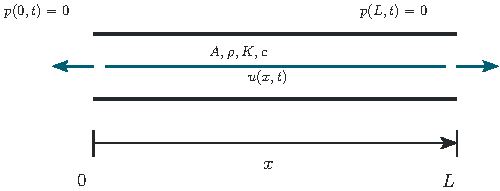
\includegraphics[width=0.84\linewidth]{figures/generated/solutions/C2-tube.pdf}
\caption{Open--open tube used for the analysis. The ends are at $x=0$ and $x=L$.}
\label{fig:hw02-c2-tube}
\end{figure}

\textbf{2. Boundary conditions.} At each open end the pressure disturbance vanishes.
\[
\boxed{p(0,t)=0},\qquad \boxed{p(L,t)=0}.
\]
Using $p=-K u_x$, these are equivalently $U'(0)=0$ and $U'(L)=0$ for the spatial mode.

\textbf{3. Harmonic displacement solution.} Separation of variables gives
\[
\boxed{u(x,t)=U(x)e^{-i\omega t}},\qquad
\boxed{U(x)=C_1\sin(\gamma x)+C_2\cos(\gamma x)}.
\]

\textbf{4. Pressure--displacement relation.} The pressure disturbance is related to the axial strain by
\[
\boxed{p(x,t)=-K\frac{\partial u}{\partial x}}.
\]

\textbf{5. Pressure in terms of $C_1$ and $C_2$.} Differentiating the displacement field gives
\[
\boxed{p(x,t)=-K\gamma\left[C_1\cos(\gamma x)-C_2\sin(\gamma x)\right]e^{-i\omega t}}.
\]

\begin{samepage}
\textbf{6. Boundary equations.} Substitution into the boundary conditions gives
\[
p(0,t)=-K\gamma C_1e^{-i\omega t}=0,
\]
\[
p(L,t)=-K\gamma\left[C_1\cos(\gamma L)-C_2\sin(\gamma L)\right]e^{-i\omega t}=0.
\]
\end{samepage}

\textbf{7. Constants.} The first equation gives $C_1=0$. The second equation then becomes
\[
\boxed{C_2\sin(\gamma L)=0}.
\]

\textbf{8. Trivial solution.} If $C_2=0$, then $C_1=0$ also, so $U(x)=0$, $u(x,t)=0$, and $p(x,t)=0$. This is the fluid at rest and contains no vibration.

\textbf{9. Nontrivial solution.} For vibration, take $C_2\ne0$. The wavenumber must therefore satisfy
\[
\boxed{\sin(\gamma L)=0}.
\]

\textbf{10. Eigenvalue equation.} With $z=\gamma L$,
\[
\boxed{\sin z=0}.
\]

\textbf{11. Eigenvalues.} The positive acoustic roots are
\[
\boxed{z_j=j\pi},\qquad j=1,2,3,\ldots.
\]
The root $z=0$ gives $\gamma=0$, $\omega=0$, and a spatially constant displacement. It is a non-vibratory rigid motion with zero pressure and is excluded from the acoustic mode index.

\textbf{12. Wavenumbers.} Since $z_j=\gamma_jL$,
\[
\boxed{\gamma_j=\frac{j\pi}{L}}.
\]

\textbf{13. Wavenumber definition.} The wavenumber is related to angular frequency by
\[
\boxed{\gamma=\frac{\omega}{c}}.
\]

\textbf{14. Angular frequency.} Solving the preceding relation for frequency gives
\[
\boxed{\omega=\gamma c}.
\]

\textbf{15. Natural angular frequencies.} Substituting $\gamma_j$ gives
\[
\boxed{\omega_j=\frac{j\pi c}{L}}.
\]

\textbf{16. Frequencies in hertz.} Since $\omega_j=2\pi f_j$,
\[
\boxed{f_j=\frac{jc}{2L}}.
\]

\textbf{17. Fundamental and overtones.} The fundamental frequency is $f_1=c/(2L)$. The overtones are the higher resonant frequencies, with $f_j=jf_1$.

\textbf{18. Harmonics.} The fundamental is the first harmonic. The open--open tube supports all integer harmonics, so the first overtone is the second harmonic, the second overtone is the third harmonic, and so on.

\textbf{19. Wavelength relation.} Wavenumber and wavelength satisfy
\[
\boxed{\lambda=\frac{2\pi}{\gamma}}.
\]

\textbf{20. Modal wavelengths.} Using the wavenumbers above,
\[
\boxed{\lambda_j=\frac{2L}{j}}.
\]

\textbf{21. Wavelength multiples.} Rearranging the last expression gives
\[
\boxed{L=j\frac{\lambda_j}{2}}.
\]
Thus the tube contains $j$ half-wavelengths. Both ends are displacement antinodes and pressure nodes. Mode $j$ has $j$ interior displacement nodes and $j-1$ interior pressure nodes; its pressure field has $j$ interior antinodes.

\textbf{22. Elimination of $C_1$.} From item 7, $C_1=0$, so
\[
\boxed{U(x)=C_2\cos(\gamma x)}.
\]

\textbf{23. Displacement modeshapes.} Choosing the arbitrary scale $C_2=1$ gives
\[
\boxed{U_j(x)=\cos(\gamma_jx)=\cos\left(\frac{j\pi x}{L}\right)}.
\]

\textbf{24. Normalized displacement modeshapes.} The first five modes are plotted against $\xi=x/L$ in Figure~\ref{fig:hw02-c2-disp}. Every mode has displacement antinodes at $\xi=0$ and $\xi=1$. The five modes fit one, two, three, four, and five half-wavelengths into the tube. Mode $j$ has $j$ interior displacement nodes and $j+1$ displacement antinodes, including both ends.

\begin{figure}[H]
\centering
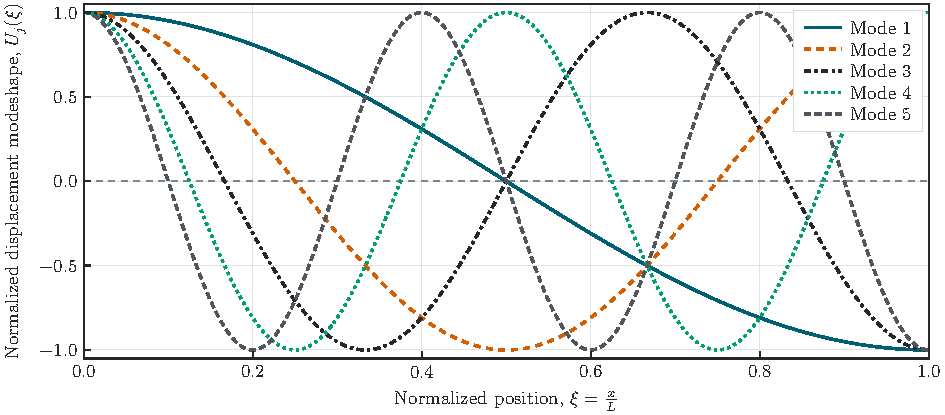
\includegraphics[width=0.96\linewidth]{figures/generated/solutions/C2-modes.pdf}
\caption{Normalized displacement modeshapes $U_j(\xi)=\cos(j\pi\xi)$ for the first five open--open tube modes.}
\label{fig:hw02-c2-disp}
\end{figure}

\textbf{25. Graduate work.} Let $a_j>0$ denote the displacement amplitude in meters. Using $u_j(x,t)=a_jU_j(x)e^{-i\omega_jt}$ with $p=-Ku_x$ gives
\[
p_j(x,t)=K a_j\gamma_j\sin(\gamma_jx)e^{-i\omega_jt}.
\]
Normalizing by the peak pressure amplitude $K a_j\gamma_j$ gives
\[
\boxed{\bar P_j(\xi)=\sin(j\pi\xi)}.
\]
The pressure modeshapes are plotted in Figure~\ref{fig:hw02-c2-pressure}. The open ends are pressure nodes and displacement antinodes. Mode $j$ has $j-1$ interior pressure nodes and $j$ interior pressure antinodes. The positive sign follows directly from differentiating $U_j$ in the relation $p=-Ku_x$.

\begin{figure}[H]
\centering
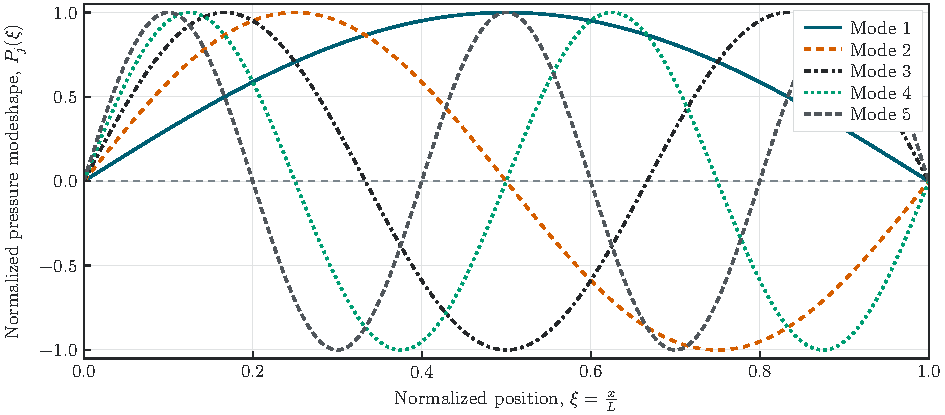
\includegraphics[width=0.96\linewidth]{figures/generated/solutions/C2-pressure.pdf}
\caption{Normalized pressure modeshapes $\bar P_j(\xi)=\sin(j\pi\xi)$ for the first five open--open tube modes.}
\label{fig:hw02-c2-pressure}
\end{figure}

\clearpage
\matlabcaption{MATLAB plots for C.2.}
\lstinputlisting[style=hwmatlab]{matlab/C2.m}
